\section{任务计划}
\subsection{选题}
\begin{itemize}
    \item 线路负载及故障检测装置(2019年C题)
    \item 简易频率特性测试仪(2013年E题)
    \item 自适应滤波器(2017年E题)
    \item 远程幅频特性测试装置(可选,2017年H题)
\end{itemize}

\subsection{任务分析}
在一、二、四题中均需要制作信号源,其中线路负载检测和简易频率特性测试两题均要求
同时获得待测网络的幅频和相频特性,用于显示频率特性或进一步判断其拓扑结构。
因此可以使用双相位法,该方法基本流程如下:

\begin{figure}[H]
\center
    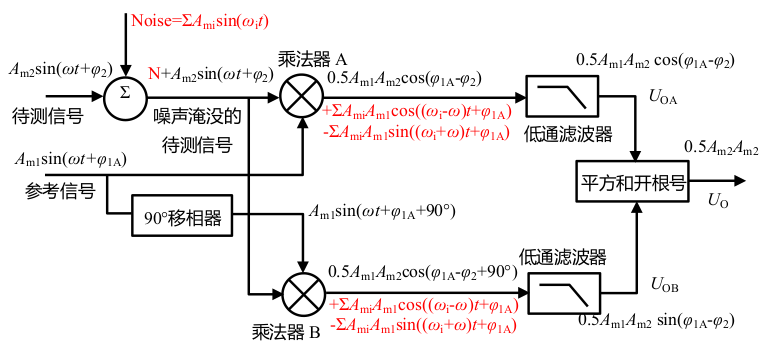
\includegraphics[width=\textwidth]{img/biphasic.png}
    \captionof{figure}{双相位锁定放大器基本原理}
\end{figure}

该方法要求产生两路正交信号,分别和待测信号相乘,经低通滤波后与另一路输出计算平方和再开根号,
便可以取得待测信号的幅度,同时可以进一步根据$U_\textrm{OA}$和$U_\textrm{OB}$求得参考信号和待测信号的相位差:
\begin{equation}
    \varphi_\textrm{1A}-\varphi_\textrm{2} =
    \arctan{\dfrac{U_\textrm{OB}}{U_\textrm{OA}}}
\end{equation}

信号的输出端为直流信号,考虑到失调电压的影响和反正切函数的非线性,一点测量误差可能带来较大的
相位计算偏差,因此需要高精度ADC进行采样;失调电压则可在上电时进行校准,或使用零失调运放。

自适应滤波器一题的软件部分相对较少,使用定时器捕获测量出干扰源信号频率即可。

远程幅频特性中也需要用到信号发生源,但并不要求正交输出,因此在前面几题的基础上可较容易地实现。

\subsection{器件选型}
ADI公司的DDS信号发生器AD9854可以支持双路正交信号输出,最高时钟频率可达\SI{300}{MHz},
因此可以作为较理想的正交信号发生源;直流信号测量的精确度要求较高,
可以选用TI公司的24位ADC:ADS124S08,该器件支持12路差分或单端输入,
采样率在\SI{2.5}{SPS}到\SI{4000}{SPS}之间可调。

在远程幅频特性测试装置的要求中,信号源的输出范围是\SI{1}{MHz}$\sim$\SI{40}{MHz},
而对AD9854的初步测试发现,器件在PLL参考时钟倍频数较低时,尚未达到\SI{40}{MHz}的输出时
便已出现了明显的欠采样现象;倍频数较高时,虽然能达到最高输出频率的要求,但器件功耗也大大增加,
稳定性下降,甚至出现偶尔无法正常复位的问题。因此针对该选题我们可能需要考察输出频率更高的DDS,
如AD9910,其最大输出频率能达到\SI{400}{MHz}.

微控制器则选用STM32H743系列,其工作频率可达\SI{480}{MHz},外设数量、端口也十分丰富,
为很多应用带来了更高的精度、更低的延时。

人机交互方面,原本打算使用STM32H7开发板自带的5寸电容屏,经过初步测试也能正常工作,
但是考虑到几点因素,最终决定不使用:

\begin{enumerate}
    \item 占用引脚过多。控制该显示屏需要使用的外设:SDRAM、LTDC、FMC,一共占用八十余个引脚,
    严重挤占其他外设的分配;
    \item 例程与我们的器件配置差别较大,很难直接移植,因此需重新开发一个基于事件回调的GUI系统,
    或者使用现成的框架。前者和核心算法并不相干,不值得投入大量时间;
    后者考察了LVGL等嵌入式GUI库,最终发现链接出来的二进制文件过大,
    考虑到后期核心应用也会占用大量代码空间,因此保险起见不予使用。
\end{enumerate}

最终决定选用广州大彩的组态串口屏DC10600GM070\_1111\_1T,相较于单片机在像素级别完全控制液晶屏,
该显示屏自带上位机,可自行处理点击、刷新等事件,我们只需要维护单片机与其的UART通讯,
处理好事件回调、命令发送等任务即可,大大降低了单片机的工作量。同时,该组态屏的界面设计可以借助
图形化的IDE来完成,十分方便。

综上,需要驱动编写的器件清单如下:

\begin{enumerate}
    \item DDS信号源:AD9854、AD9910
    \item ADC:ADS124S08
    \item 串口屏:DC10600GM070\_1111\_1T
\end{enumerate}
